\chapter{Results}
\label{chap:results}


All results are obtained on a PC with an AMD FX-9590, 16 GB RAM and an AMD Radeon HD 7970. 


\section{Shape Detection Benchmarking}

The interactions proposed in this thesis heavily rely on the ability to detect meaningful shapes for regions of interest within interactive time. Therefore it must be assured that the shape detection provides results within interactive time such that the detected shapes can be used immediately for interactions. Section \ref{sec:shapedetectionperformance} discusses the performance obtained in the test computer. 


\section{Performance}
\label{sec:shapedetectionperformance}

The goal of the \textit{user-guided shape detection} is to provide meaningful results within interactive time, such that detected shapes can be used to support interactions immediately. The capabilities of the implementation by Schnabel et. al\cite{schnabel-2007-software} are benchmarked on three different datasets: 

\begin{center}
\begin{tabular}{ l | r | r | r }

		& 										\textbf{\#Points} 				& \textbf{\#Nodes} 	& \textbf{max. LoD} \\
		\hline
  JB\_Haus.pts									& 620.722 								& 440 			& 15 \\
  Technologiezentrum\_Teil1.pts	& 11.762.924							& 8863 			& 15 \\
  Synthetic\_Primitives.pts 		& 472.000 								& 315	 			& 5 \\
	
\end{tabular}
\end{center}

The testing methodology works without user interaction. Instead, all octree nodes are collected and fed into the shape detection routine sequentially in order to retrieve results for each node of the point cloud. Therefore, the shape detection is performed for the complete point cloud for each \textit{level-of-detail}. Each octree node contains at most 5000 points. The results are averaged over five runs. Table \ref{table:schnabel_benchmarks} shows the results averaged over all nodes. It can be seen that detecting planes only is significantly faster than detecting all types of primitive shapes. However, detecting all types of primitive shapes still produces results within interactive time. The synthetic point cloud is constructed from a set of primitives that are discretized to point sets, such that all types of primitives exist. 

\begin{table}
	\centering
	\begin{tabular}{ l || r | r | r || r | r | r}
			&\multicolumn{3}{c||}{\textbf{\#Shapes}} & \multicolumn{3}{c}{\textbf{Time (s)}}\\
			&\textbf{min} & \textbf{max} & \textbf{avg}  & \textbf{min} & \textbf{max} & \textbf{avg}  \\
			\hline
			JB\_Haus*							& 0 & 6  & 1.31 & 0.000026 & 0.578664 & 0.022396 \\
			JB\_Haus 							& 0 & 6  & 1.40 & 0.000024 & 0.741384 & 0.093264 \\
			Technologiezentrum*		& 0 & 10 & 1.18 & 0.000023 & 0.440614 & 0.018781 \\
			Technologiezentrum 		& 0 & 10 & 1.19 & 0.000024 & 0.991554 & 0.083180 \\
			Synthetic*						& 0 & 7  & 1.89 & 0.000026 & 0.440064 & 0.029779 \\
			Synthetic 						& 0 & 7  & 1.24 & 0.000024 & 0.753345 & 0.136474 \\
		\end{tabular}
	\caption{Performance measures for the different datasets averaged over all nodes. The number of shapes and duration are listed as minimum, maximum and average. Each dataset is benchmarked using plane detection only (items with *), as well as detecting all types of primitive shapes. }
	\label{table:schnabel_benchmarks}
\end{table}

\begin{figure}[h]
    \centering
    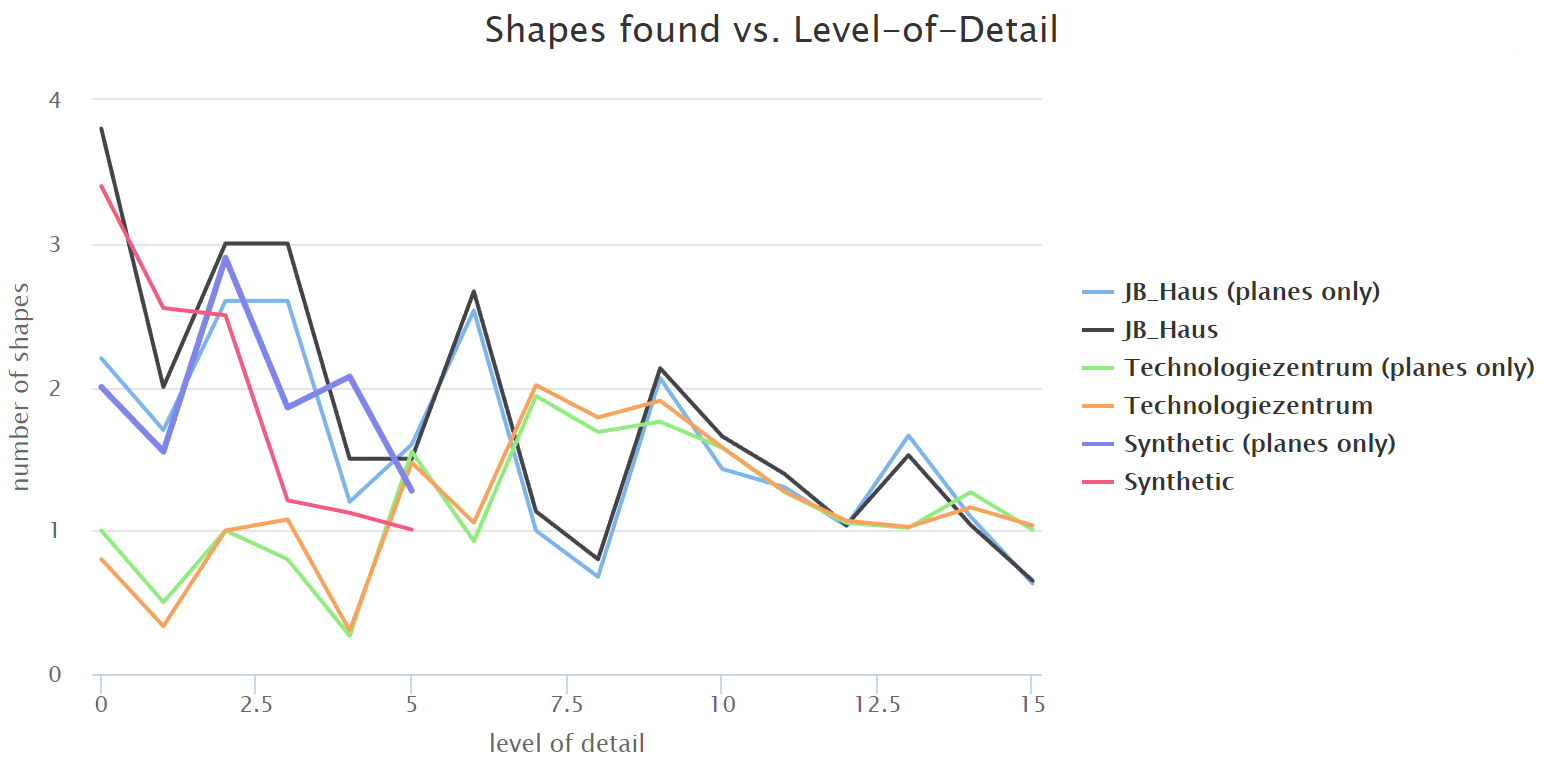
\includegraphics[width=1\textwidth]{Results/shapes_vs_lod.png}
    \caption{Plot of the number of shapes in correlation to the \textit{level-of-detail} of the node. All values are averaged over all nodes that share the same \textit{level-of-detail}.}
    \label{fig:shapes_vs_lod}
\end{figure}

\begin{figure}[h]
    \centering
    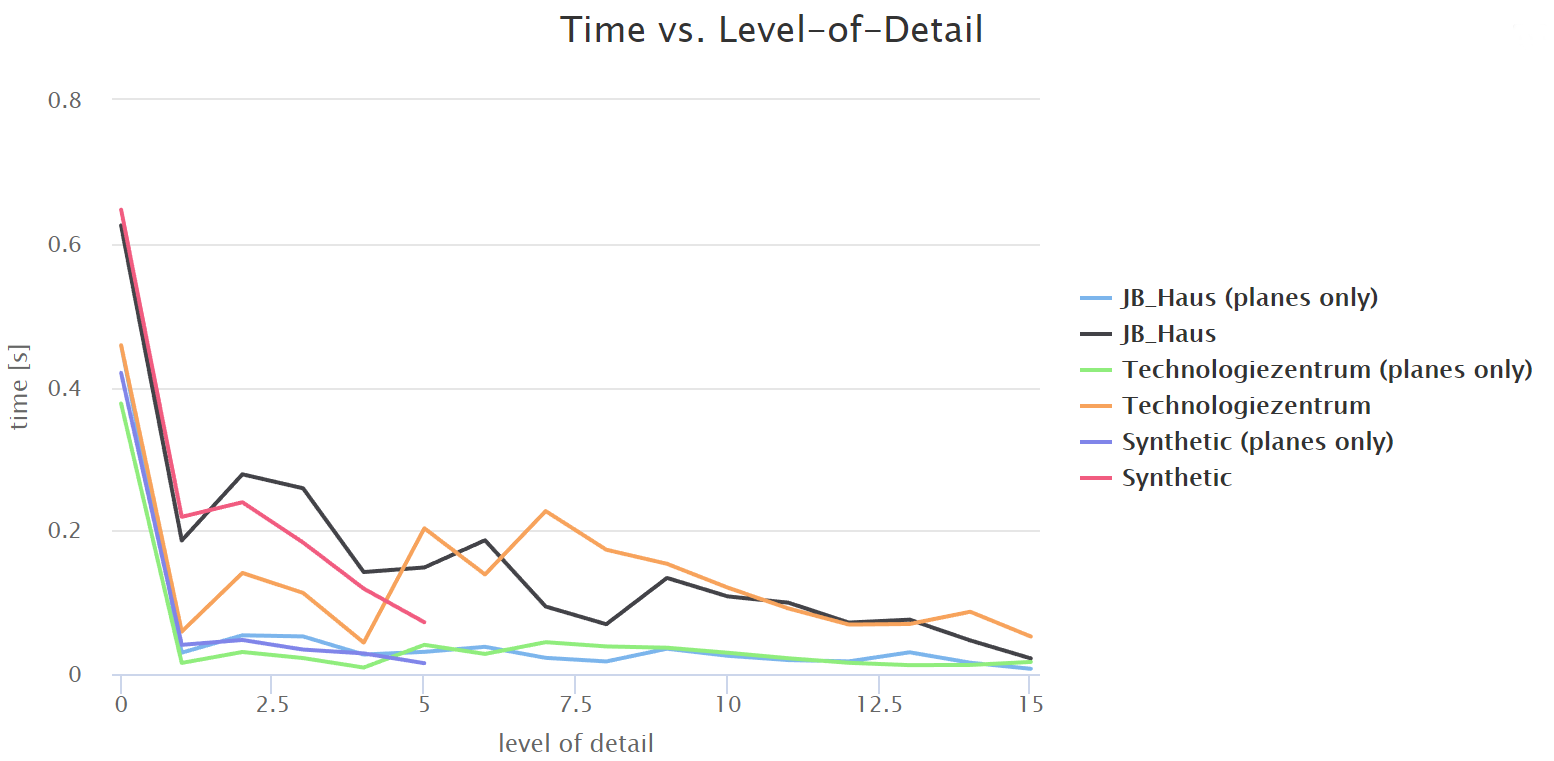
\includegraphics[width=1\textwidth]{Results/time_vs_lod.png}
    \caption{Plot of the number of shapes in correlation to the \textit{level-of-detail} of the node. All values are averaged over all nodes that share the same \textit{level-of-detail}.}
    \label{fig:time_vs_lod}
\end{figure}

Figure \ref{fig:shapes_vs_lod} shows a plot for each dataset that compares the average number of shapes per node to the \textit{level-of-detail}. The plot of the synthetic point cloud ends at 5 since it only contains 5 \textit{level-of-detail}. A trend can be seen in this plot, such that the number of shapes decreases the higher the \textit{level-of-detail} is. This comes as no surprise since the nodes with higher \textit{level-of-detail} are smaller in size, therefore containing less possible structures. 
\\

Figure \ref{fig:time_vs_lod} shows the calculation time compared to the \textit{level-of-detail}. Shape detection for smaller, more dense nodes take less time than for larger nodes with lower \textit{level-of-detail}. 


\subsection{Results}


\subsection{Errors and Crap \todo{}}

A problem with the shape detection implementation by Schnabel et. al\cite{schnabel-2007-software} are reoccurring non-terminations for some octree nodes, causing the shape detection coroutine to stall. To circumvent this problem, all shape detection tasks that are dispatched to the \verb|sequential computation applicator| are assigned a timeout value of one second, after which the computation is interrupted. 
\\
Another reoccurring problem with the shape detection is the plausibility of detected shapes. The RANSAC options guarantee that shapes are found that fit the local geometry within a certain margin, $\alpha$ for the normal's angle and $\epsilon$ for the distance the the shape. So within theses two parameters, the shape is considered to be valid. However, certain constellation of points allow the shape detection to produce non-plausible results that valid in terms of the RANSAC shape detection, but are not plausible to the eye. A prominent example is a torus that is fitted onto a section that clearly describes a cylinder. The major radius of the torus is at such dimensions that the local cylinder fits within the curvature of the torus, thus a torus is detected, rather than the simpler cylinder. Figure \ref{fig:missfittedTorus} shows this behavior within an example scene that consists multiple primitives. Figure \ref{fig:missfittedTorus2} shows the size of the detected torus. 
\\
The reason such non-plausible shapes exist is the density-controlled $\epsilon$ parameter, weakening the margin for octree nodes of larger volume. Even within a node, the density can strongly vary for different regions. 

\begin{figure}
\centering
\subcaptionbox{ \label{fig:missfittedTorus1}}{%
  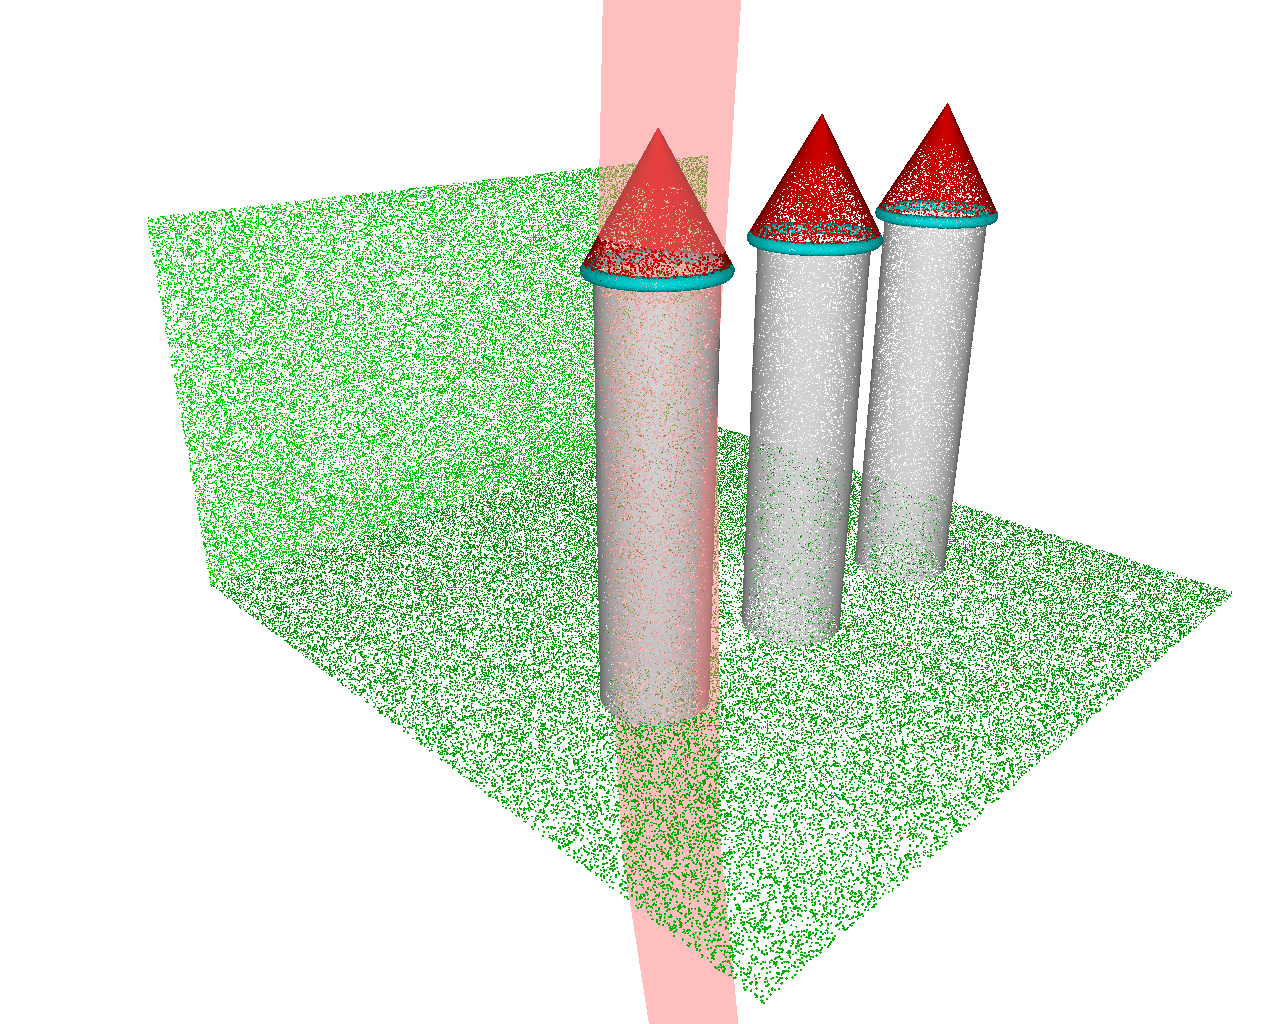
\includegraphics[width=0.49\textwidth]{Results/missfittedTorus1.png}%7
  }%\par\medskip
\subcaptionbox{ \label{fig:missfittedTorus2}}{%
  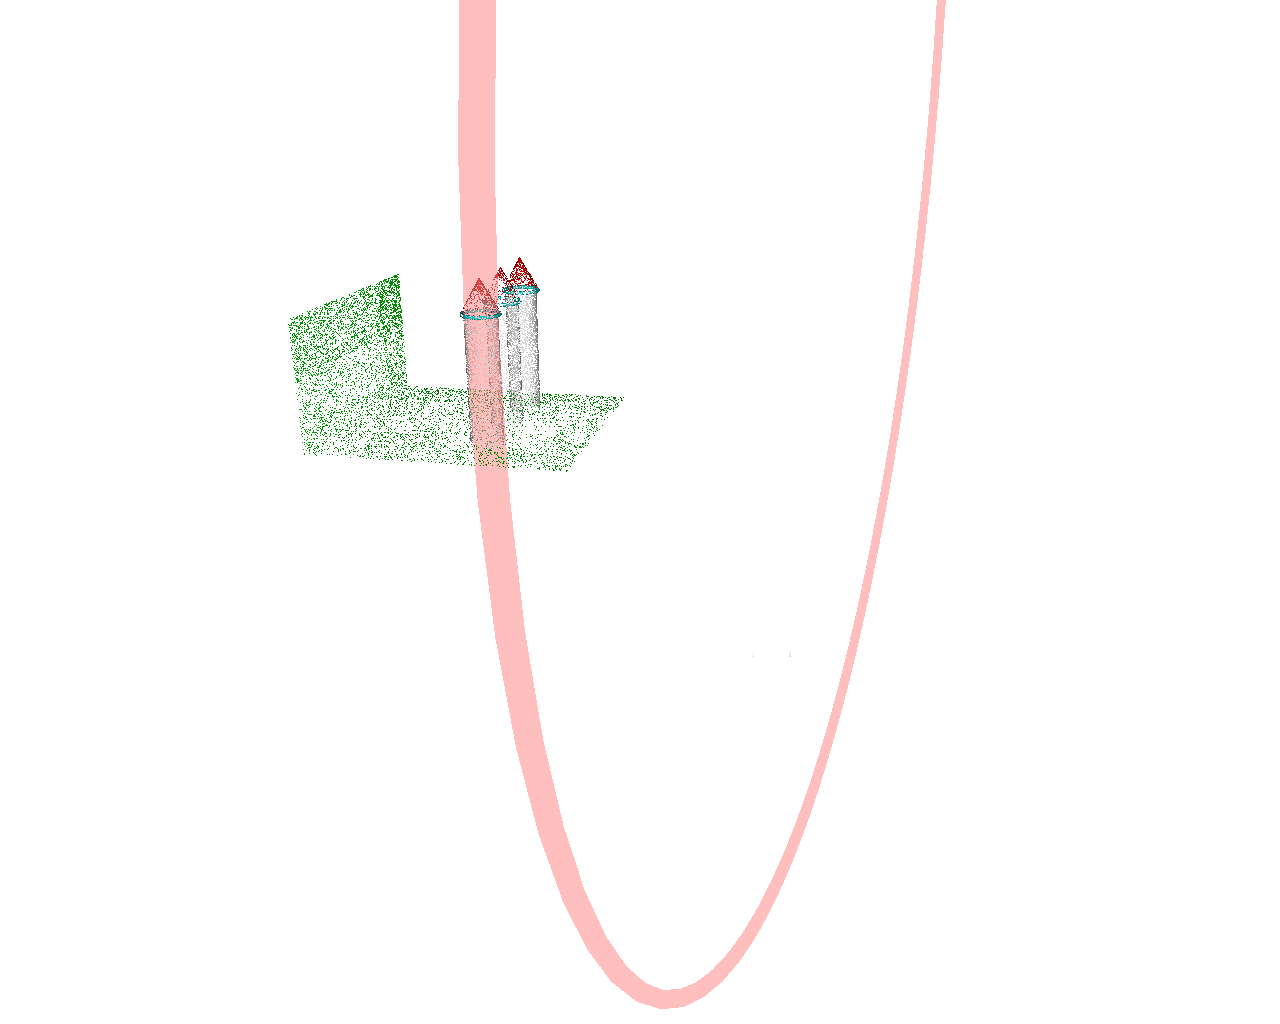
\includegraphics[width=0.49\textwidth]{Results/missfittedTorus2.png}%
  }    

  
\caption{This figure shows a synthetic cylinder in the foreground whose points are classified as a torus instead of a cylinder. Eventough the points fit the torus, determined by the RANSAC options, the result is not plausible, since the user would expect a cylinder for this constellation of points. }
\label{fig:missfittedTorus}
\end{figure}



